\documentclass{article}[11pt]
\usepackage{blindtext}
\usepackage{graphicx}
\usepackage{enumitem}
\usepackage{amssymb}
\usepackage{amsthm}
\usepackage{amsmath}
\usepackage{graphicx}
\usepackage{MnSymbol}
\usepackage{wasysym}
\usepackage{pgfplots}
\usepackage{tikz}
\usepackage{graphicx}
\graphicspath{ {./images/} }
\usetikzlibrary{calc}
\usetikzlibrary{shapes}
\usetikzlibrary{shapes.geometric}
\usepgfplotslibrary{fillbetween}
\pgfplotsset{width=10cm,compat=1.9}

\title{A Collection of Hand-Drawn Mathematical Diagrams for Grant Sanderson, Compiled From Barnett Yang's Multivariable Calculus Notes}
\author{Barnett Yang}
\date{April 2, 2021}

\begin{document}
\maketitle

% \begin{figure}[h]
%     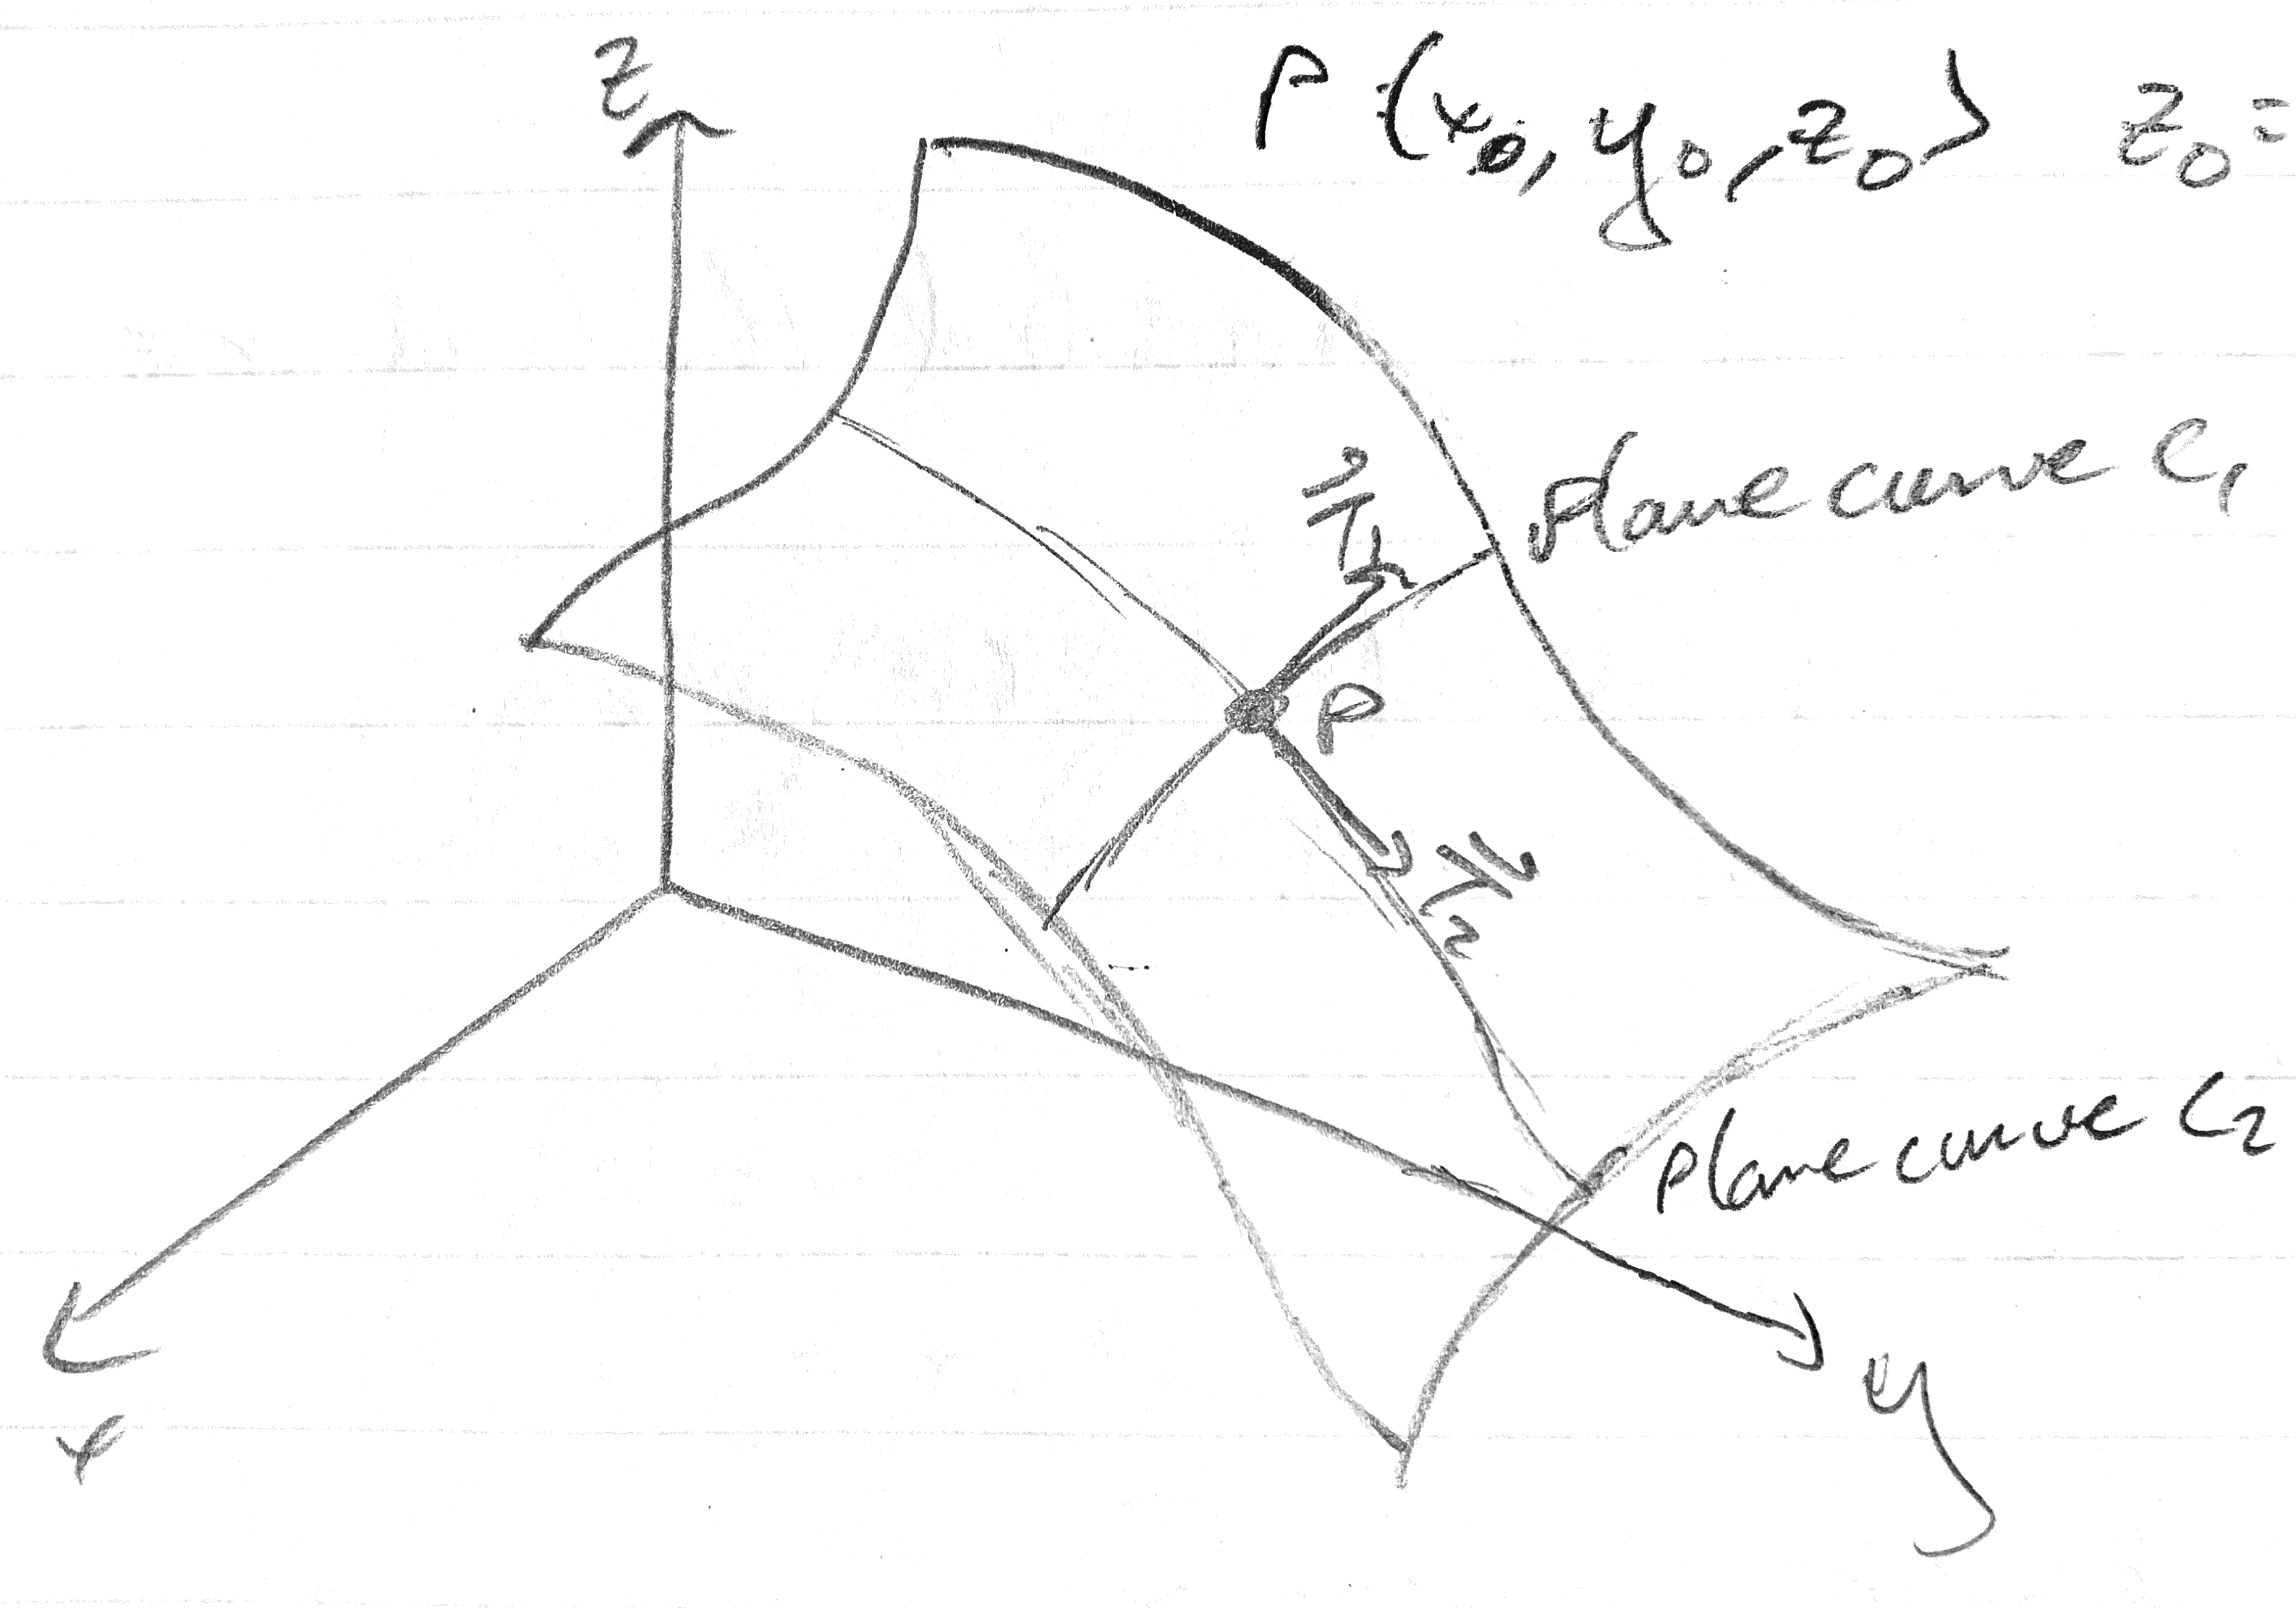
\includegraphics[width=\textwidth]{img1.PNG}
%     \caption{A plane and its two tangent vectors along two plane curves.}
% \end{figure}

\begin{figure}[h]
    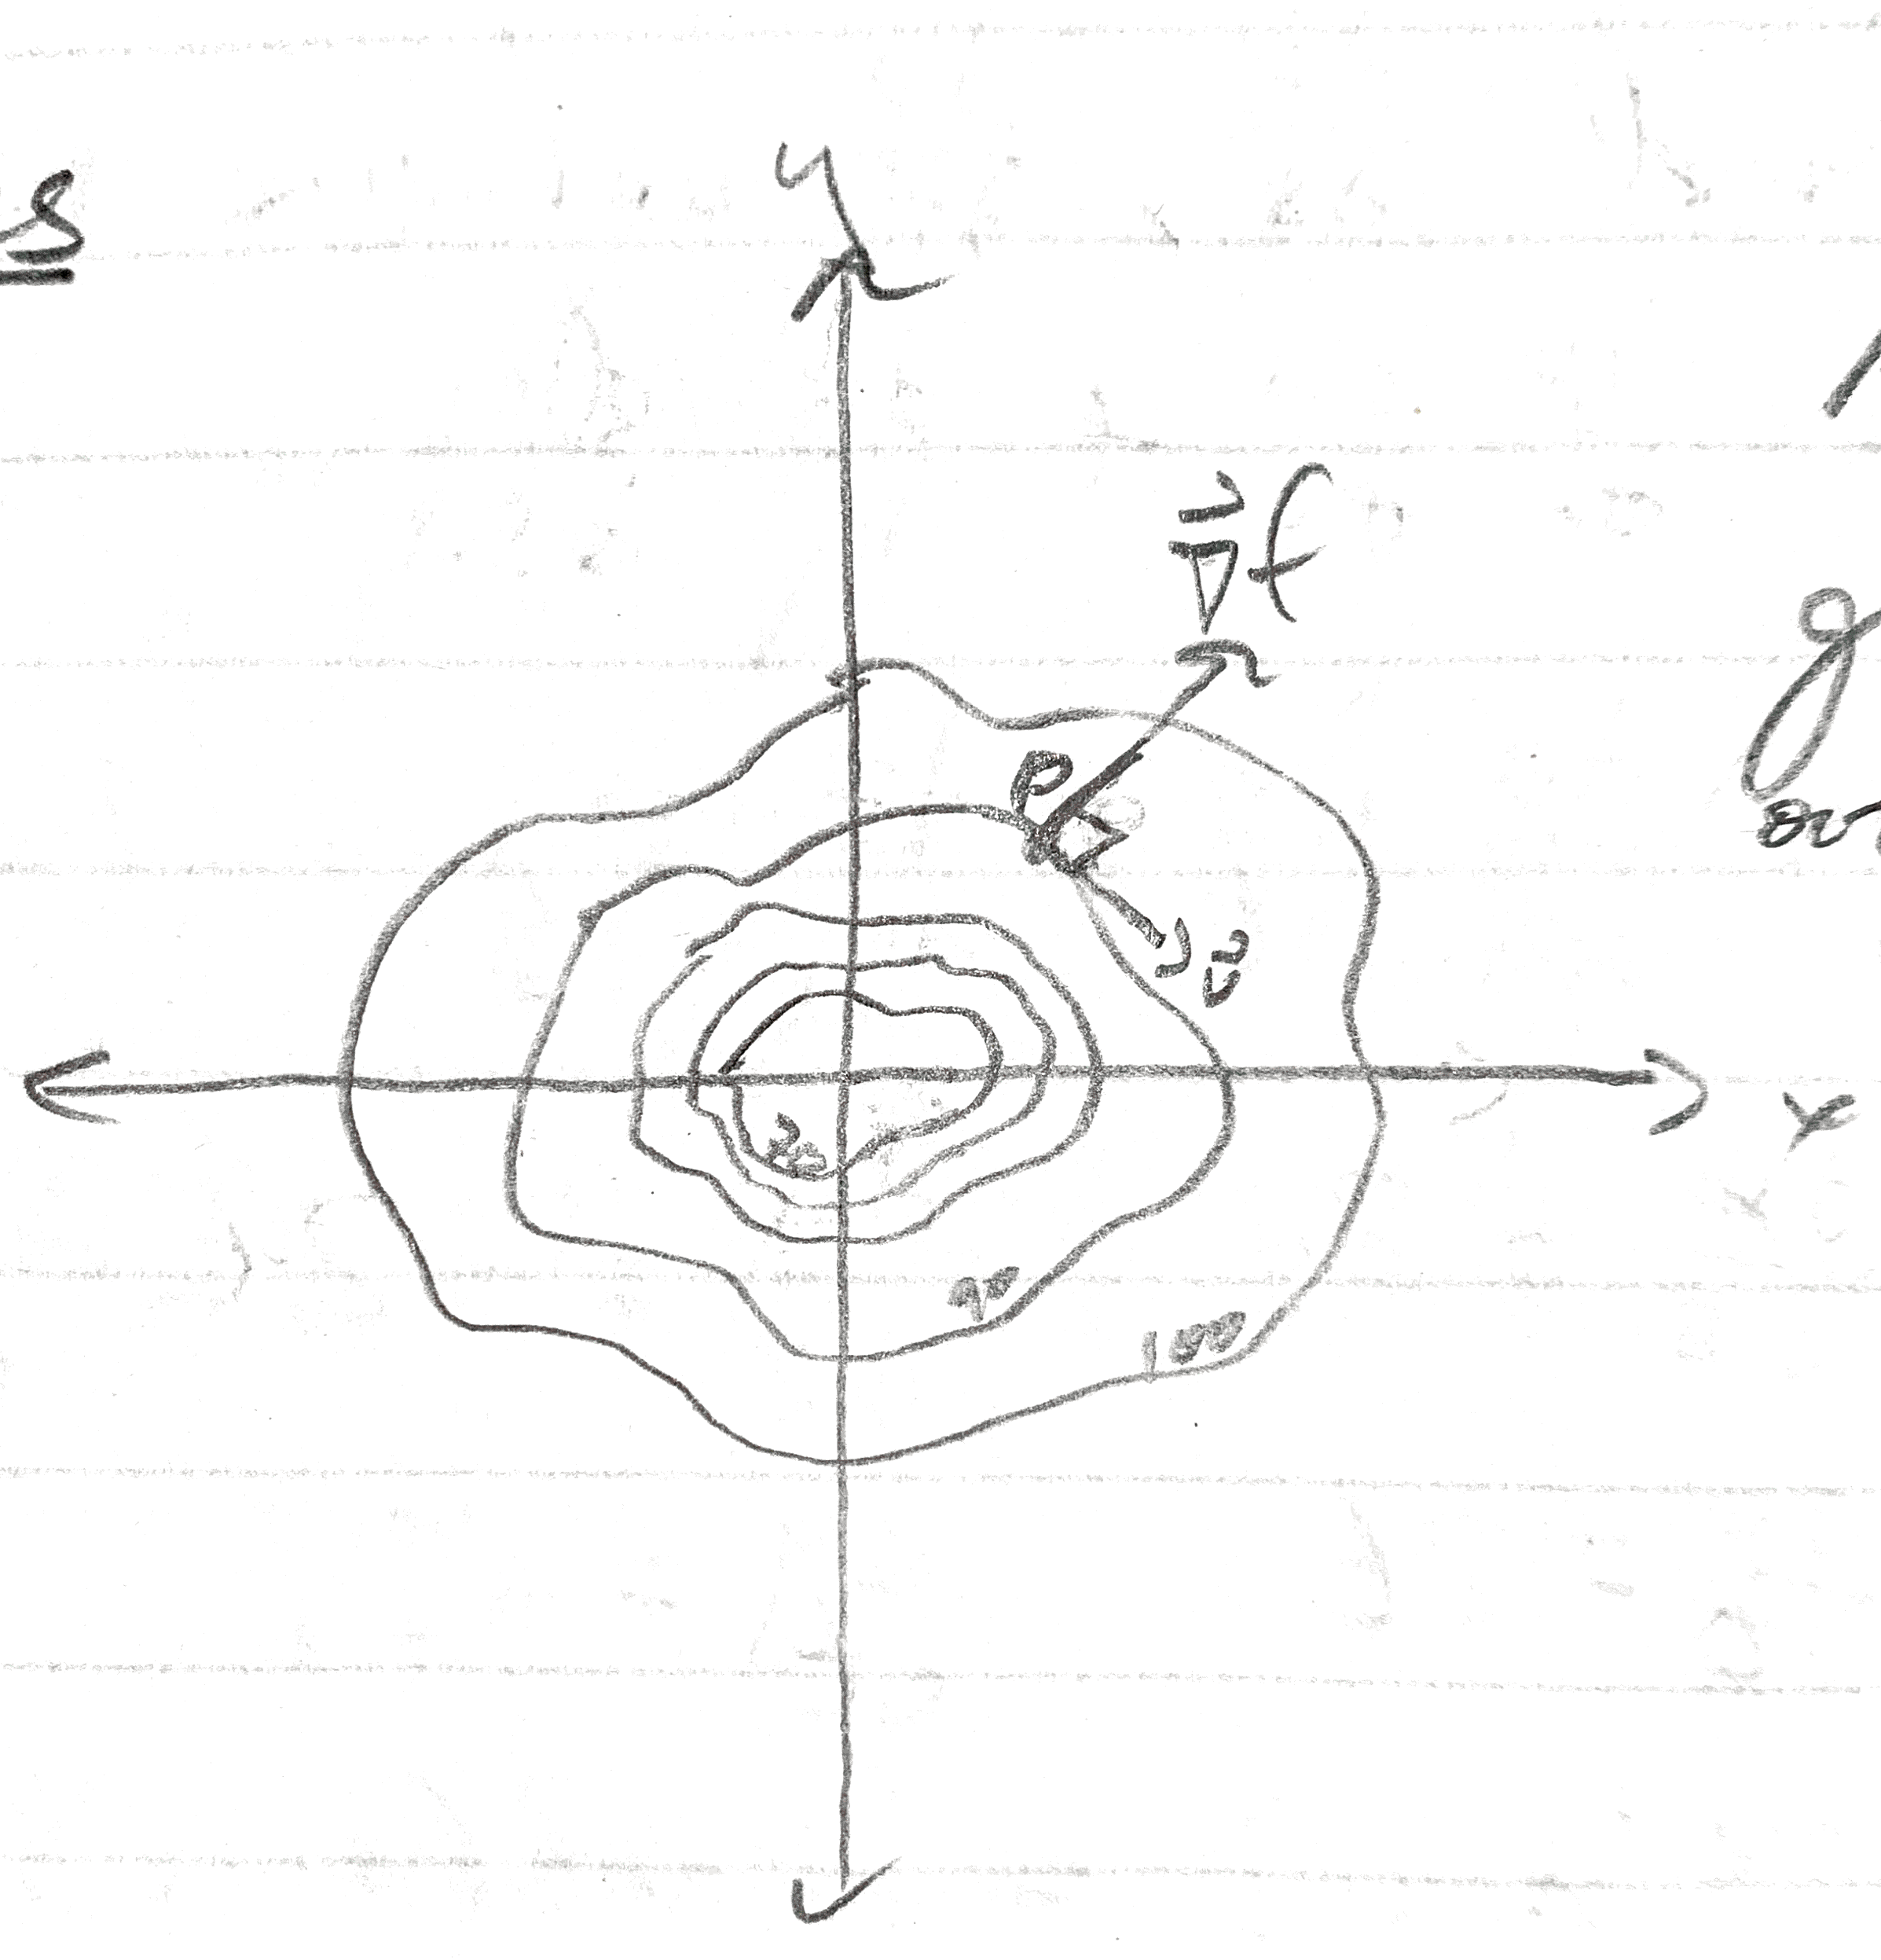
\includegraphics[width=\textwidth]{img2.PNG}
    \caption{A series of level curves and a gradient vector.}
\end{figure}

\begin{figure}[h]
    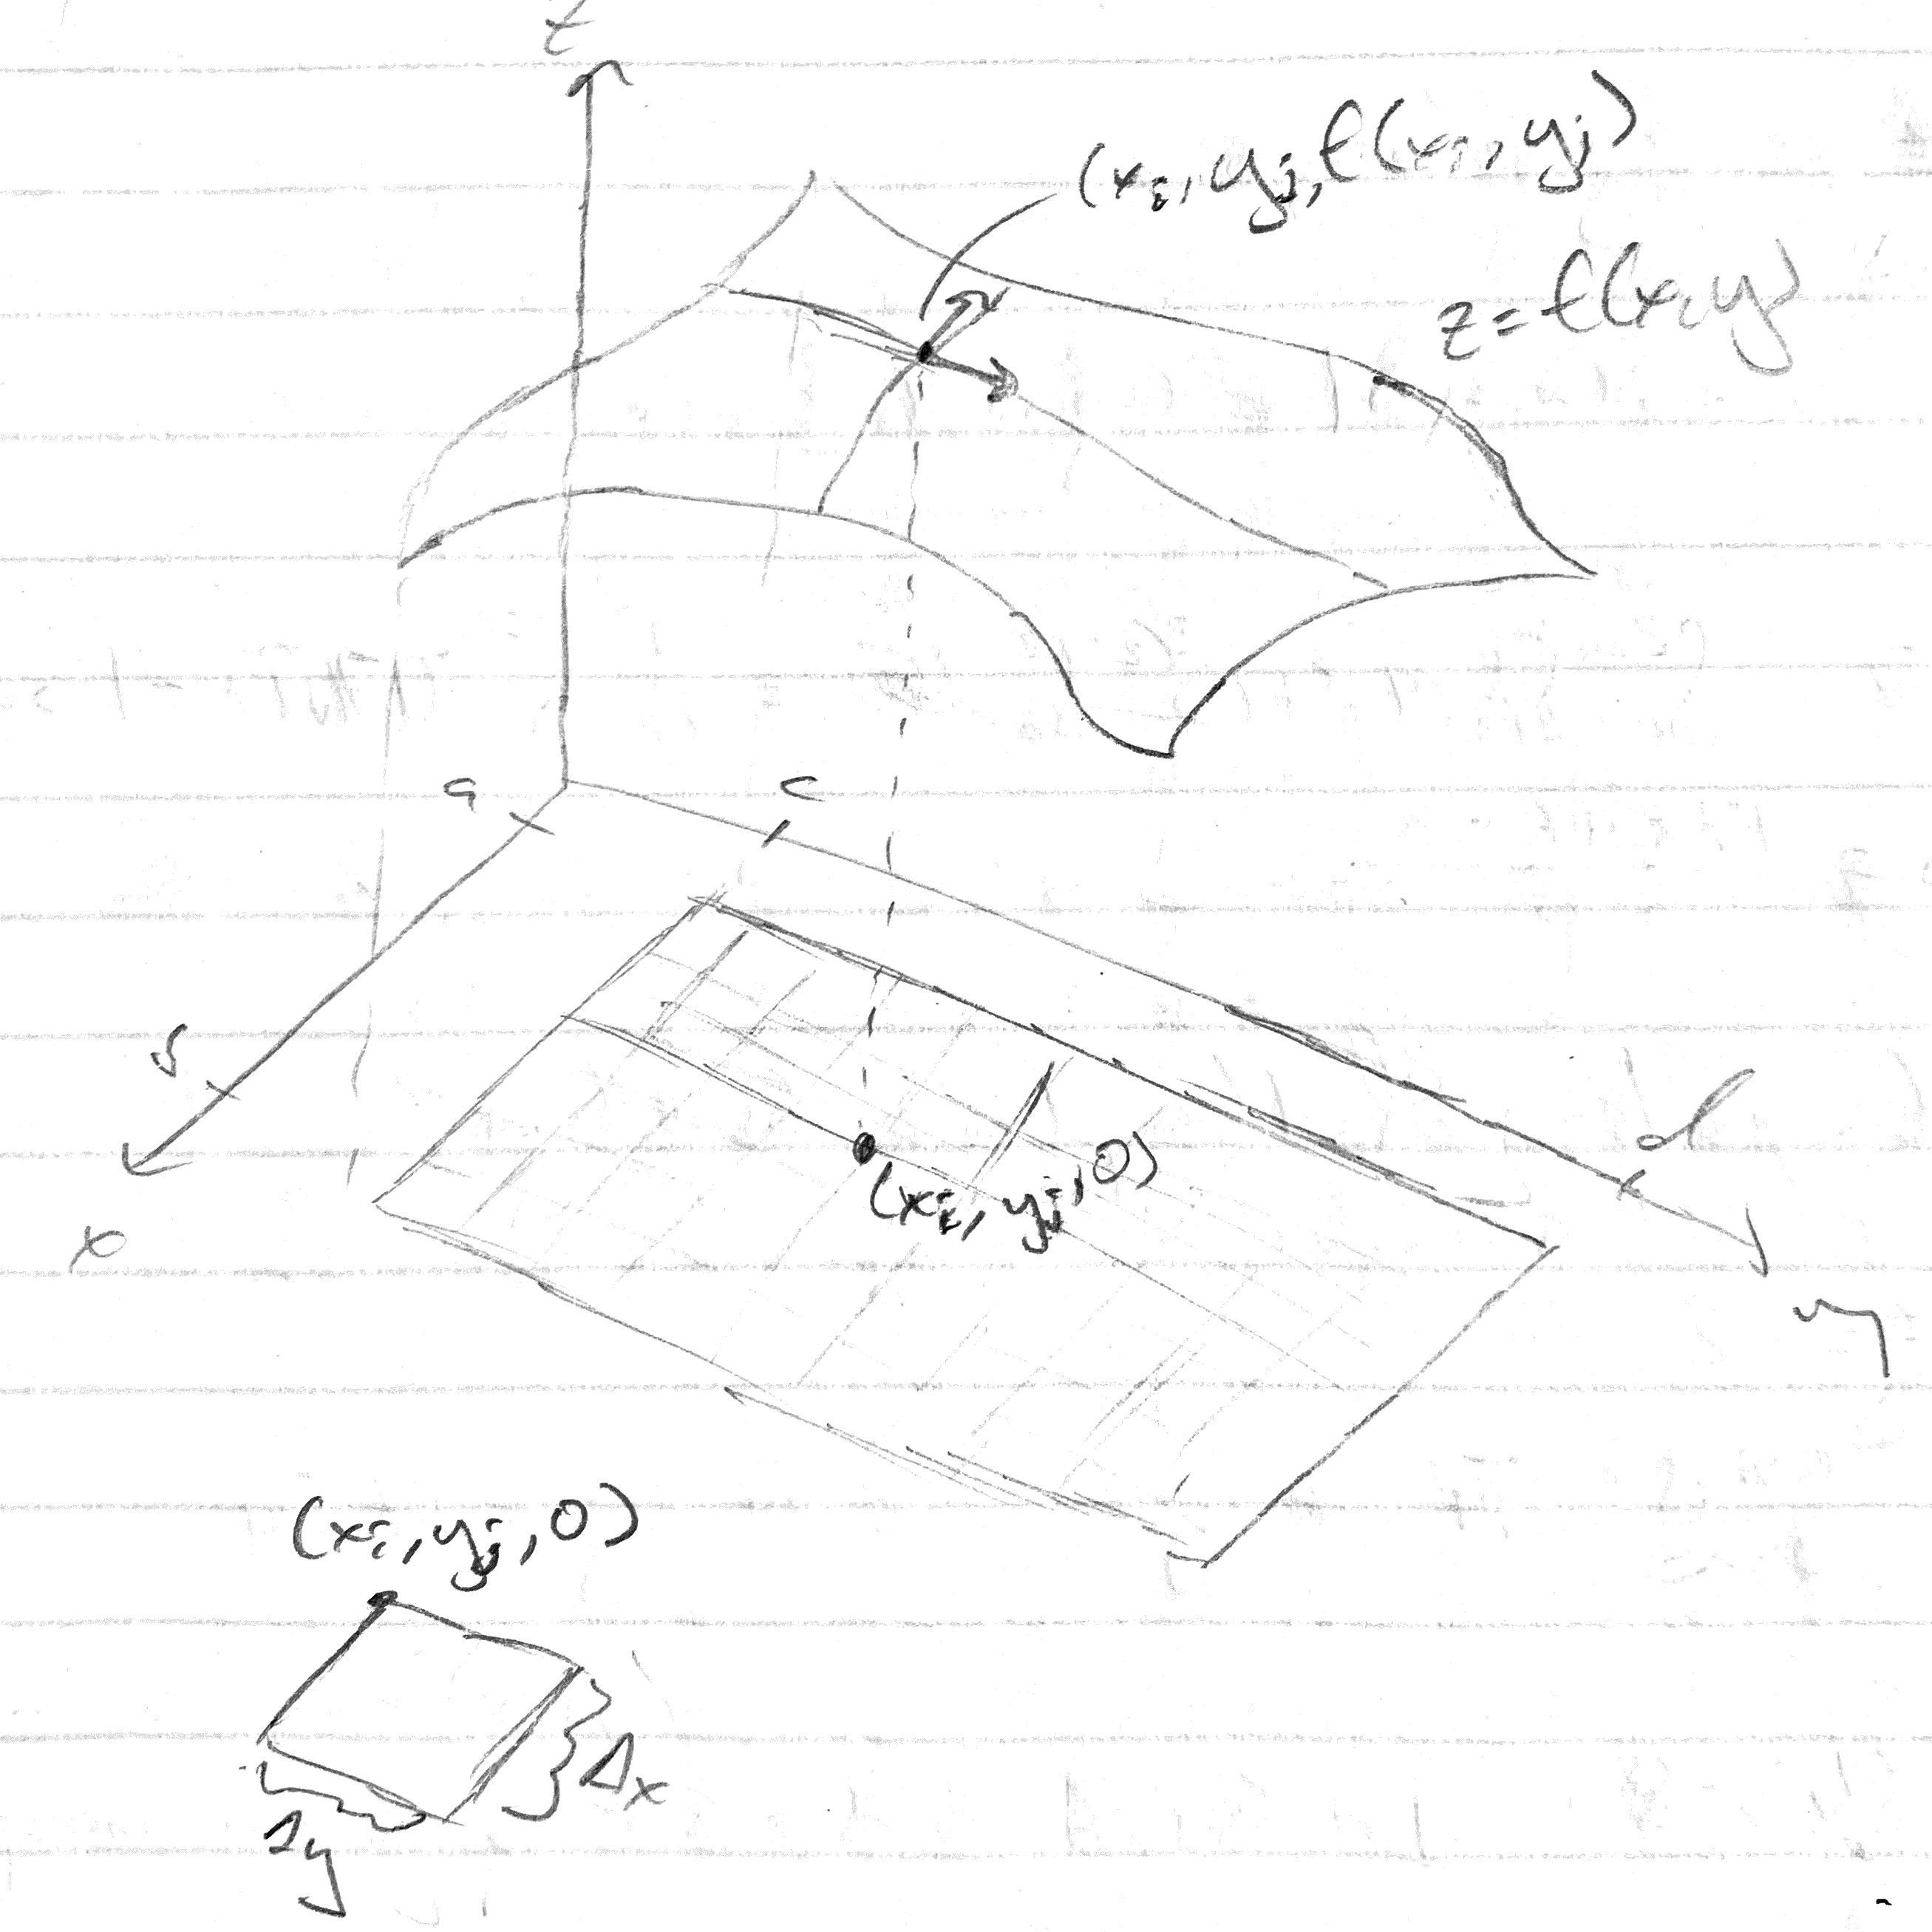
\includegraphics[width=\textwidth]{img3.PNG}
    \caption{Finding the surface area of, well, a surface.}
\end{figure}

\begin{figure}[h]
    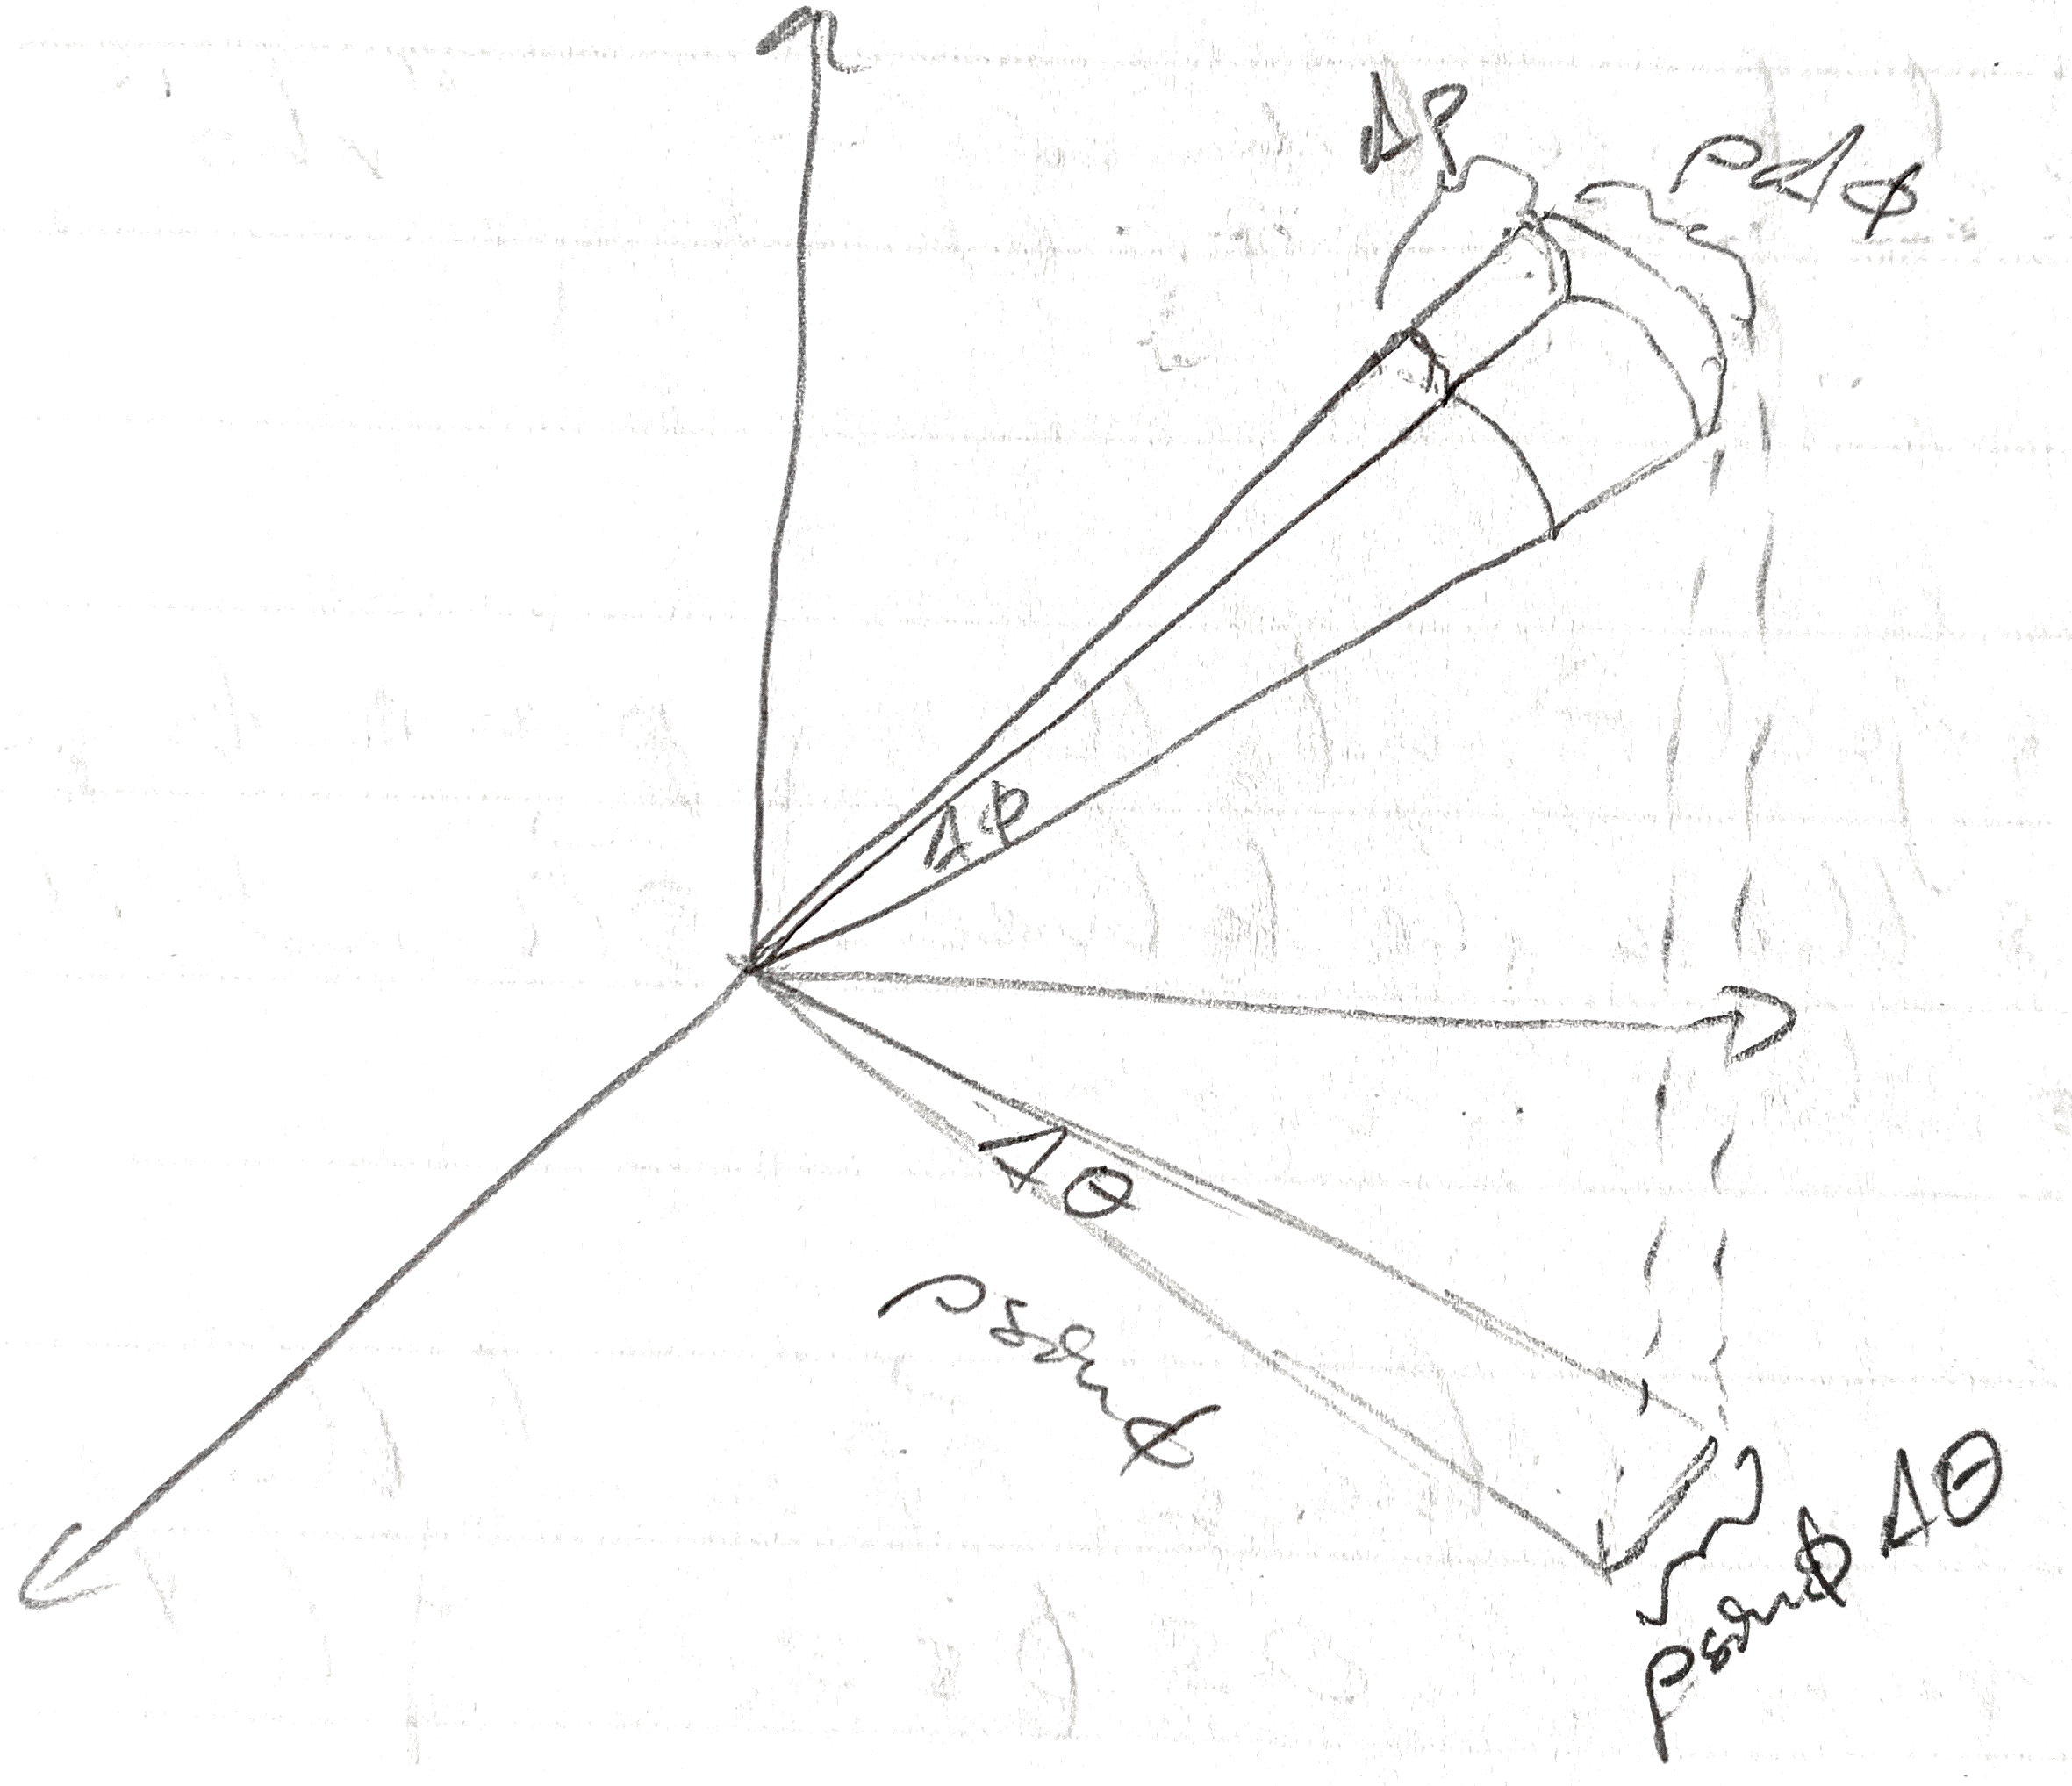
\includegraphics[width=\textwidth]{img4.PNG}
    \caption{Finding volumes using polar coordinates.}
\end{figure}

\begin{figure}[h]
    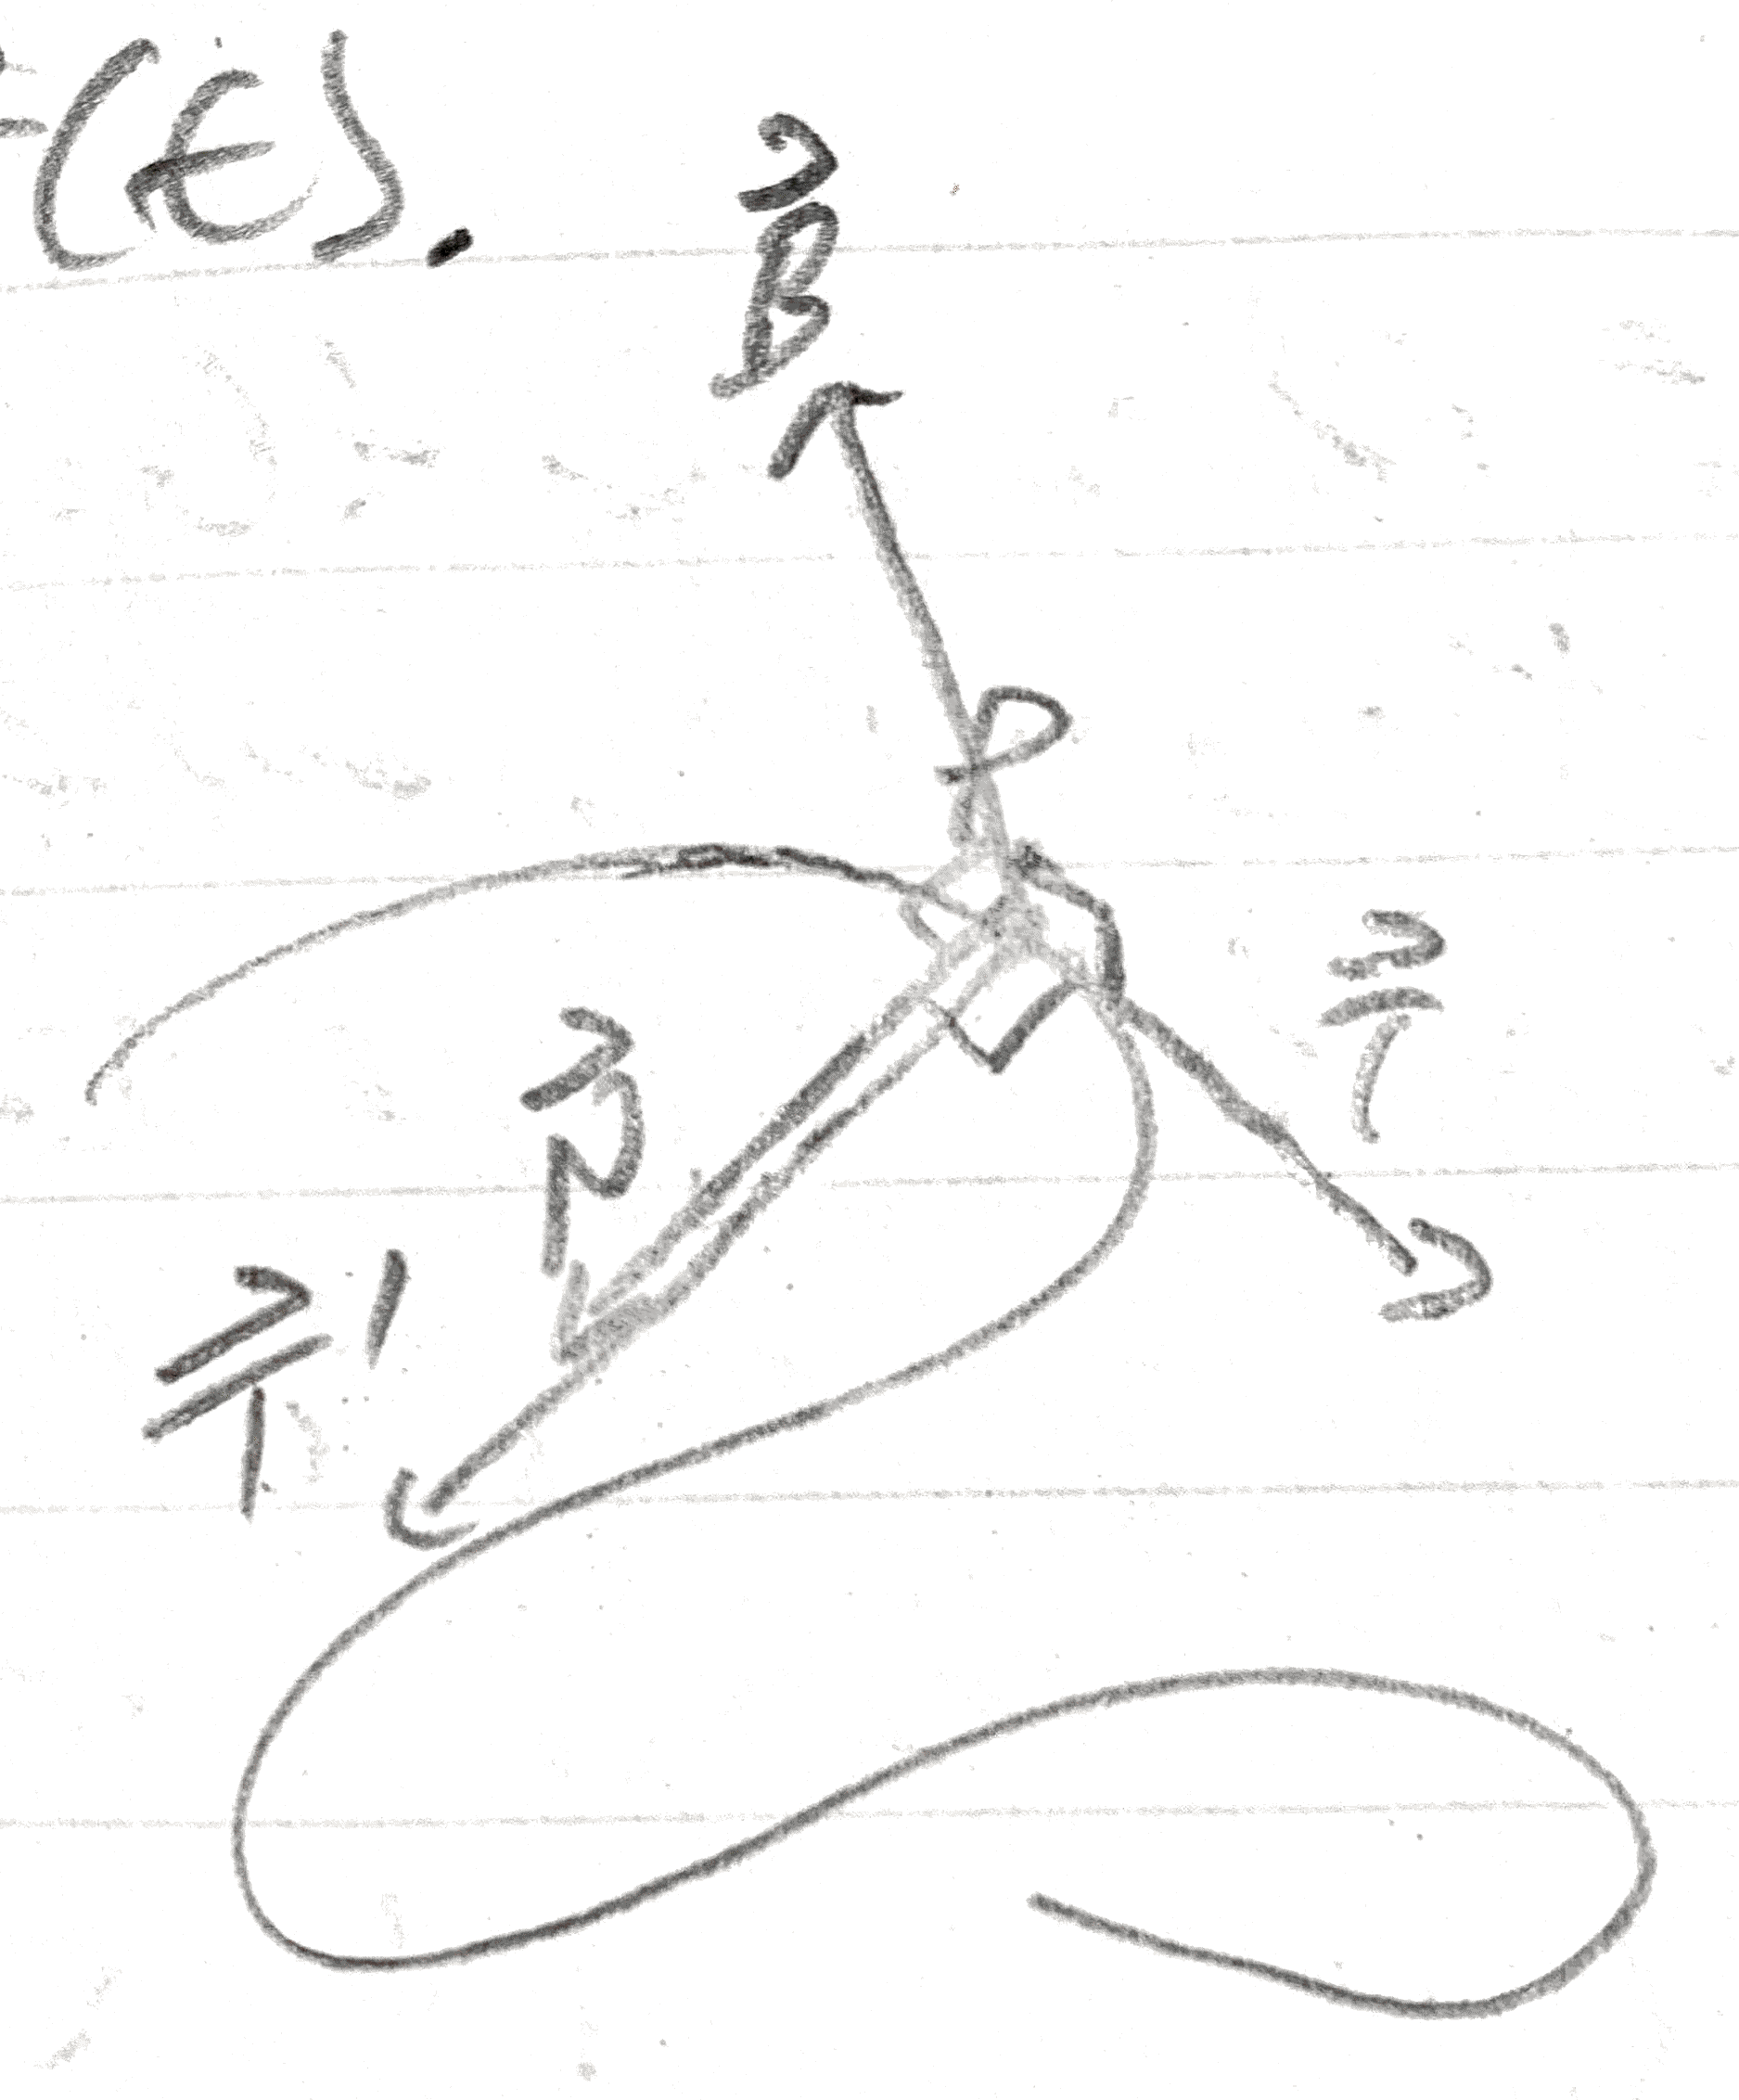
\includegraphics[width=\textwidth]{img5.PNG}
    \caption{A line vector and its derivative, normal, and binormal vectors.}
\end{figure}
\end{document}
